% !TEX program = xelatex
\documentclass[11pt, aspectratio=169]{beamer}
\usetheme{metropolis}
\useoutertheme{metropolis}
\useinnertheme{metropolis}
\usecolortheme{metropolis}
\usefonttheme{professionalfonts} 

\usepackage{kotex}
\usepackage{tikz} 
\usepackage{graphicx, caption, hyperref, fontawesome5}

% [수식 및 폰트 설정 - 기존 파일 그대로 유지]
\usepackage{amsmath}
\usepackage[math-style=ISO, bold-style=ISO]{unicode-math}

\usefonttheme{professionalfonts}

% 본문 폰트 (Pretendard)
\setmainfont[Ligatures=TeX, BoldFont={* Bold}, AutoFakeSlant=0.2]{Pretendard}
\setsansfont[Ligatures=TeX, BoldFont={* Bold}, AutoFakeSlant=0.2]{Pretendard}
\setmainhangulfont[BoldFont={* Bold}]{Pretendard}
\setsanshangulfont[BoldFont={* Bold}]{Pretendard}

% 수식 폰트 (Fira Math + Pretendard)
\setmathfont{Fira Math}
\setmathfont[range={up, bfup}, Scale=MatchLowercase]{Pretendard}
\setmathfont[range={it, bfit}, Scale=MatchLowercase, FakeSlant=0.2]{Pretendard}

% [중요] 그림 경로 수정 (슬라이드 폴더 기준 2단계 위로)
\graphicspath{{../../assets/}}

% 메타데이터 (Chapter 2로 수정)
\title{Communication Theory - 2026}
\subtitle{Chapter 2. Signals and Signal Space}
\date{\today}
\author{
    이 경 근 \\
    {\tiny
        \raisebox{-0.1ex}{\scalebox{0.85}{\faEnvelope}} \href{mailto:infosec@knu.ac.kr}{infosec@knu.ac.kr} \quad 
        {\scalebox{0.9}{\faLinkedin}} \scalebox{0.9}{\href{https://www.linkedin.com/in/Kenny-0633-Lee}{Kenny-0633-Lee}}
    }
}
\institute{EE / KNU}

%%%%%%%%%%%%%%%%%%%%%%%%%%%%%%%%%%%%%%%%%%%%%
%%%%%%%%%%%%%%%%%%%%%%%%%%%%%%%%%%%%%%%%%%%%%

\begin{document}

% 1. 표지
\begin{frame}[plain]
    \titlepage
\end{frame}

% 2. 강의 목차
\begin{frame}{Chapter 2 Overview}
    \begin{itemize}
        \item \textbf{Basic Signals:} 단위 계단 함수 $u(t)$와 델타 함수 $\delta(t)$
        \item \textbf{Signal Operations:} 시간 이동(Shifting)과 스케일링(Scaling)
        \item \textbf{Correlation:} 신호의 유사도(Similarity) 측정
    \end{itemize}
\end{frame}

% 3. 기본 신호 (Unit Step)
\begin{frame}{1. Basic Signals: Unit Step Function}
    \begin{columns}
        \begin{column}{0.6\textwidth}
            \centering
            % Python(ch02_signals.py)에서 생성한 그림
            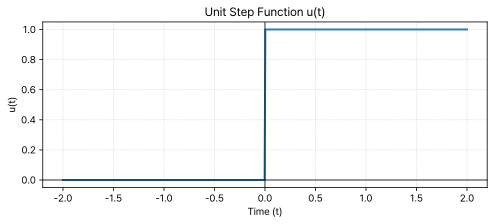
\includegraphics[width=\textwidth]{fig_ch02_unit_step.pdf}
        \end{column}
        \begin{column}{0.4\textwidth}
            \begin{block}{Definition}
                \[
                u(t) = \begin{cases} 
                1, & t \ge 0 \\ 
                0, & t < 0 
                \end{cases}
                \]
            \end{block}
            \vspace{0.2cm}
            \textbf{Key Property:} \\
            시스템의 스위칭 동작(Switching)을 수학적으로 모델링할 때 사용됨.
        \end{column}
    \end{columns}
\end{frame}

% 4. 신호의 연산 (Shifting & Scaling)
\begin{frame}{2. Signal Operations: $x(at - b)$}
    \begin{columns}
        \begin{column}{0.55\textwidth}
            \centering
            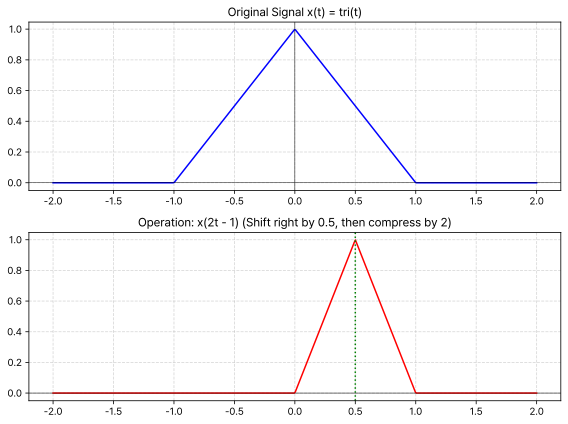
\includegraphics[width=\textwidth]{fig_ch02_operations.pdf}
        \end{column}
        \begin{column}{0.45\textwidth}
            \small
            \textbf{해석 순서 (Order of Operations):}
            \begin{enumerate}
                \item \textbf{Shifting:} $t \rightarrow t - t_0$ \\
                (Right if $t_0 > 0$)
                \item \textbf{Scaling:} $t \rightarrow at$ \\
                (Compression if $a > 1$)
            \end{enumerate}
            
            \vspace{0.3cm}
            \begin{alertblock}{Caution}
                $x(2t - 1)$은 $x(t)$를 1만큼 이동 후 2배 압축하는 것이 아님! \\
                $\rightarrow x(2(t - 0.5))$로 생각해야 함.
            \end{alertblock}
        \end{column}
    \end{columns}
\end{frame}

% 5. 상관관계 (Correlation)
\begin{frame}{3. Signal Correlation}
    \centering
    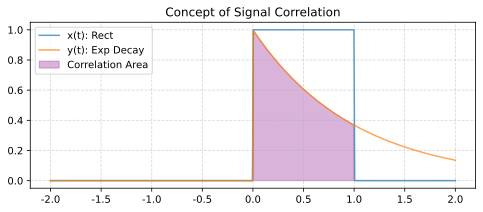
\includegraphics[width=0.7\textwidth]{fig_ch02_correlation.pdf}
    
    \vspace{0.3cm}
    \begin{block}{Correlation Coefficient ($C_n$)}
        두 신호가 얼마나 닮았는가? (Measure of Similarity)
        \[
        \rho = \frac{\int x(t) y^*(t) dt}{\sqrt{E_x E_y}}
        \]
    \end{block}
    \small \textit{그래프의 보라색 영역(Overlap)이 넓을수록 상관관계가 높습니다.}
\end{frame}

% 6. 마무리
\begin{frame}{Summary}
    \begin{itemize}
        \item \textbf{Unit Step $u(t)$:} 인과성(Causality) 표현의 핵심
        \item \textbf{Operations:} $x(at-b)$ 꼴의 변환을 자유자재로 다뤄야 함
        \item \textbf{Correlation:} 통신 시스템에서 수신 신호를 검출(Detection)하는 기본 원리
    \end{itemize}
\end{frame}

\end{document}